%!TEX program = xelatex

\documentclass[a4paper, openany, oneside]{memoir}
\usepackage[no-math]{fontspec}
\usepackage{pgfplots}
\pgfplotsset{compat=newest}
\usepackage{commath}
\usepackage{mathtools}
\usepackage{amssymb}
\usepackage{amsthm}
\usepackage{booktabs}
\usepackage{mathtools}
\usepackage{xcolor}
\usepackage[separate-uncertainty=true, per-mode=symbol]{siunitx}
\usepackage[noabbrev, capitalize]{cleveref}
\usepackage{listings}
\usepackage[american inductor, european resistor]{circuitikz}
\usepackage{amsmath}
\usepackage{amsfonts}
\usepackage{ifxetex}
\usepackage[dutch,english]{babel}
\usepackage[backend=bibtexu,texencoding=utf8,bibencoding=utf8,style=ieee,sortlocale=en_GB,language=auto]{biblatex}
\usepackage[strict,autostyle]{csquotes}
\usepackage{parskip}
\usepackage{import}
\usepackage{standalone}
\usepackage{hyperref}
%\usepackage[toc,title,titletoc]{appendix}

\ifxetex{} % Fonts laden in het geval dat je met Xetex compiled
    \usepackage{fontspec}
    \defaultfontfeatures{Ligatures=TeX} % To support LaTeX quoting style
    \setromanfont{Palatino Linotype} % Tover ergens in Font mapje in root.
    \setmonofont{Source Code Pro}
\else % Terug val in standaard pdflatex tool chain. Geen ondersteuning voor OTT fonts
    \usepackage[T1]{fontenc}
    \usepackage[utf8]{inputenc}
\fi
\newcommand{\references}[1]{\begin{flushright}{#1}\end{flushright}}
\renewcommand{\vec}[1]{\boldsymbol{\mathbf{#1}}}
\newcommand{\uvec}[1]{\boldsymbol{\hat{\vec{#1}}}}
\newcommand{\mat}[1]{\boldsymbol{\mathbf{#1}}}
\newcommand{\fasor}[1]{\boldsymbol{\tilde{\vec{#1}}}}
\newcommand{\cmplx}[0]{\mathrm{j}}
\renewcommand{\Re}[0]{\operatorname{Re}}
\newcommand{\Cov}{\operatorname{Cov}}
\newcommand{\Var}{\operatorname{Var}}
\newcommand{\proj}{\operatorname{proj}}
\newcommand{\Perp}{\operatorname{perp}}
\newcommand{\col}{\operatorname{col}}
\newcommand{\rect}{\operatorname{rect}}
\newcommand{\sinc}{\operatorname{sinc}}
\newcommand{\IT}{\operatorname{IT}}
\newcommand{\F}{\mathcal{F}}

\newtheorem{definition}{Definition}
\newtheorem{theorem}{Theorem}


\DeclareSIUnit{\voltampere}{VA} %apparent power
\DeclareSIUnit{\pii}{\ensuremath{\pi}}

\hypersetup{%setup hyperlinks
    colorlinks,
    citecolor=black,
    filecolor=black,
    linkcolor=black,
    urlcolor=black
}

% Example boxes
\usepackage{fancybox}
\usepackage{framed}
\usepackage{adjustbox}
\newenvironment{simpages}%
{\AtBeginEnvironment{itemize}{\parskip=0pt\parsep=0pt\partopsep=0pt}
\def\FrameCommand{\fboxsep=.5\FrameSep\shadowbox}\MakeFramed{\FrameRestore}}%
{\endMakeFramed}

% Impulse train
\DeclareFontFamily{U}{wncy}{}
\DeclareFontShape{U}{wncy}{m}{n}{<->wncyr10}{}
\DeclareSymbolFont{mcy}{U}{wncy}{m}{n}
\DeclareMathSymbol{\Sha}{\mathord}{mcy}{"58}
\addbibresource{../../../includes/bibliography.bib}

\title{Compressive Sensing - An Overview}

\author{W.P. Bruinsma \and R.P. Hes \and H.J.C. Kroep \and T.C. Leliveld \and W.M. Melching \and T.A. aan de Wiel}

\raggedbottom

\begin{document}
\chapter{Model - The Core}
\label{cha:model}
In this chapter we will discuss the model part of our system. All functionality discussed in this chapter is contained in the \lib{spectral\_core} module.

\begin{figure*}[h]
    \centering
    \begin{adjustbox}{width=\textwidth}
    %!TEX program = xelatex

\documentclass[a4paper, openany, oneside]{memoir}
\usepackage[no-math]{fontspec}
\usepackage{pgfplots}
\pgfplotsset{compat=newest}
\usepackage{commath}
\usepackage{mathtools}
\usepackage{amssymb}
\usepackage{amsthm}
\usepackage{booktabs}
\usepackage{mathtools}
\usepackage{xcolor}
\usepackage[separate-uncertainty=true, per-mode=symbol]{siunitx}
\usepackage[noabbrev, capitalize]{cleveref}
\usepackage{listings}
\usepackage[american inductor, european resistor]{circuitikz}
\usepackage{amsmath}
\usepackage{amsfonts}
\usepackage{ifxetex}
\usepackage[dutch,english]{babel}
\usepackage[backend=bibtexu,texencoding=utf8,bibencoding=utf8,style=ieee,sortlocale=en_GB,language=auto]{biblatex}
\usepackage[strict,autostyle]{csquotes}
\usepackage{parskip}
\usepackage{import}
\usepackage{standalone}
\usepackage{hyperref}
%\usepackage[toc,title,titletoc]{appendix}

\ifxetex{} % Fonts laden in het geval dat je met Xetex compiled
    \usepackage{fontspec}
    \defaultfontfeatures{Ligatures=TeX} % To support LaTeX quoting style
    \setromanfont{Palatino Linotype} % Tover ergens in Font mapje in root.
    \setmonofont{Source Code Pro}
\else % Terug val in standaard pdflatex tool chain. Geen ondersteuning voor OTT fonts
    \usepackage[T1]{fontenc}
    \usepackage[utf8]{inputenc}
\fi
\newcommand{\references}[1]{\begin{flushright}{#1}\end{flushright}}
\renewcommand{\vec}[1]{\boldsymbol{\mathbf{#1}}}
\newcommand{\uvec}[1]{\boldsymbol{\hat{\vec{#1}}}}
\newcommand{\mat}[1]{\boldsymbol{\mathbf{#1}}}
\newcommand{\fasor}[1]{\boldsymbol{\tilde{\vec{#1}}}}
\newcommand{\cmplx}[0]{\mathrm{j}}
\renewcommand{\Re}[0]{\operatorname{Re}}
\newcommand{\Cov}{\operatorname{Cov}}
\newcommand{\Var}{\operatorname{Var}}
\newcommand{\proj}{\operatorname{proj}}
\newcommand{\Perp}{\operatorname{perp}}
\newcommand{\col}{\operatorname{col}}
\newcommand{\rect}{\operatorname{rect}}
\newcommand{\sinc}{\operatorname{sinc}}
\newcommand{\IT}{\operatorname{IT}}
\newcommand{\F}{\mathcal{F}}

\newtheorem{definition}{Definition}
\newtheorem{theorem}{Theorem}


\DeclareSIUnit{\voltampere}{VA} %apparent power
\DeclareSIUnit{\pii}{\ensuremath{\pi}}

\hypersetup{%setup hyperlinks
    colorlinks,
    citecolor=black,
    filecolor=black,
    linkcolor=black,
    urlcolor=black
}

% Example boxes
\usepackage{fancybox}
\usepackage{framed}
\usepackage{adjustbox}
\newenvironment{simpages}%
{\AtBeginEnvironment{itemize}{\parskip=0pt\parsep=0pt\partopsep=0pt}
\def\FrameCommand{\fboxsep=.5\FrameSep\shadowbox}\MakeFramed{\FrameRestore}}%
{\endMakeFramed}

% Impulse train
\DeclareFontFamily{U}{wncy}{}
\DeclareFontShape{U}{wncy}{m}{n}{<->wncyr10}{}
\DeclareSymbolFont{mcy}{U}{wncy}{m}{n}
\DeclareMathSymbol{\Sha}{\mathord}{mcy}{"58}
\addbibresource{../../../includes/bibliography.bib}
\raggedbottom

\begin{document}
\begin{tikzpicture}
    \usetikzlibrary{arrows,automata,calc}
    \tikzset{
        state/.style={
            rectangle,
            draw=black, very thick,
            minimum height=2em,
            inner sep=2pt,
            text centered,
            anchor=north,
        },
    }
    \tikzstyle{dashedd} = [anchor=north, rectangle, inner sep=5pt, draw=black, very thick, dashed]
    \tikzstyle{fancyarrow} = [draw=black, very thick, ->, auto]
    \tikzstyle{textnodes} = [align=center]

    \node[dashedd] (model) at (0, 0) {
        \begin{tikzpicture}
            \node at (0,1) {\textbf{Model}};

            \node[state, minimum height=1.5cm, minimum width=3cm] (source) at (0, 0) {
                \begin{tabular}{c}
                    \textbf{Source}\\
                    \midrule
                    \func{generate()} \\
                \end{tabular}
            };

            \node[state, minimum height=1.5cm, minimum width=3cm] (sampler) at (4, 0) {
                \begin{tabular}{c}
                    \textbf{Sampler}\\
                    \midrule
                    \func{sample()} \\
                \end{tabular}
            };

            \node[state, minimum height=1.5cm, minimum width=3cm] (reconstructor) at (8, 0) {
                \begin{tabular}{c}
                    \textbf{Reconstructor}\\
                    \midrule
                    \func{reconstruct()} \\
                \end{tabular}
            };

            \node[state, minimum height=1.5cm, minimum width=3cm] (detector) at (12, 0) {
                \begin{tabular}{c}
                    \textbf{Detector}\\
                    \midrule
                    \func{detect()} \\
                \end{tabular}
            };

            \path [fancyarrow] (source) -- node {} (sampler);
            \path [fancyarrow] (sampler) -- node {} (reconstructor);
            \path [fancyarrow] (reconstructor) -- node {} (detector);
            
        \end{tikzpicture}
    };
\end{tikzpicture}
\end{document}

    \end{adjustbox}
    \caption{The model and its components}
    \label{fig:model-diagram}
\end{figure*}

\cref{fig:model-diagram} shows the model and its components. In this chapter, the various implementations of source, sampling, reconstructions will be discussed.

\section{Source}
\label{sec:source}
All our sources are derived from one base source, that defines the methods that every source should implement: the constructor and a \func{generate} function. This generate function should return the requested number of samples from a specific source. The rest of our source can be divided in two categories, the simulated sources used for testing our algorithms and real-world sources that connect to the USRPs to retrieve samples.

\begin{figure}
    \centering
    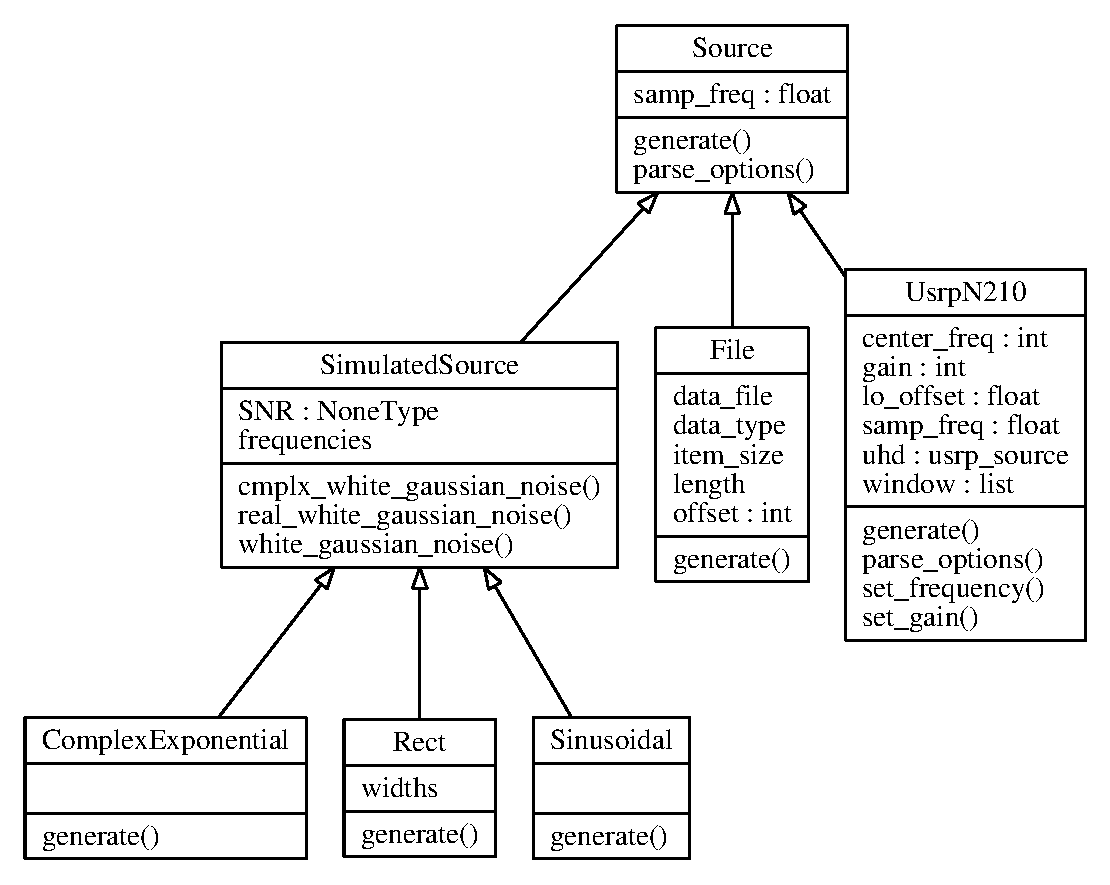
\includegraphics[width=\linewidth]{figures/classes_source.eps}
    \caption{The UML diagram of the sources}
    \label{fig:umlsource}
\end{figure}

\subsection{Simulated Source}
\label{sec:simulated-source}
The simulated sources are used for testing our algorithms. They generate samples on the fly, or use pre-recorded data. All the simulated sources have the same base class: \func{SimulatedSource}. This base class adds some utility methods to the sources to add Gaussian noise to the generated data.

\subsubsection{Sinusoidal}
The sinusoidal source generates a real valued signal, with a sum of sinusoidal signals with different frequencies. Because the signal is real valued this generates a symmetrical spectrum.

\subsubsection{Complex exponential}
The complex exponential source is the complex equivalent of the sinusoidal source. The generated complex signal is the sum of complex exponentials with different frequencies,

\subsubsection{Rectangular source}
The rectangular source generates a signal with multiple rectangles in the spectrum with specified frequencies and widths. The time domain signal is generated by adding multiple sinc functions.

\subsubsection{File source}
The file source reads the samples from a file. This was used to test with real world data, but still get reproducible results. The files can be generated with \lib{GNU Radio} using a file sink.

\subsection{USRP source}
For the USRPs we have two sources. One for normal operation for simulating different sampling methods. The other is for doing hardware co-prime sampling. The USRP sources also have methods to change the centre frequency and the gain of the front-end of the radio.

\subsubsection{Normal source}
The normal source uses the \func{finite\_acquisition} function. This provides a very easy way to get a specified number of samples from one USRP\@. This method has a few drawbacks (see \cref{sec:drivers}). The problems with the dc compensation of the local oscillator are prevented by shifting the local oscillator out of the sampled spectrum. Unfortunately this halves our effective bandwidth.

\subsubsection{Coprime source}
The coprime source uses an external \CC~program to do the actual sampling. This program synchronises the two streams and can sample from two USRPs with different sample rates. The samples are then sent over a socket to the coprime source in Python for further processing.


\section{Sampling}
\label{sec:sampling}
After the samples are generated, different sampling methods have to be applied. Each sampler implements an interface called \func{Sampler}, which has a contract for sample-method. The interface also defines a getter for the C-matrix\footnote{This is required for the reconstructors as their algorithms require knowledge about the sample intervals.}.

\begin{figure}
    \centering
    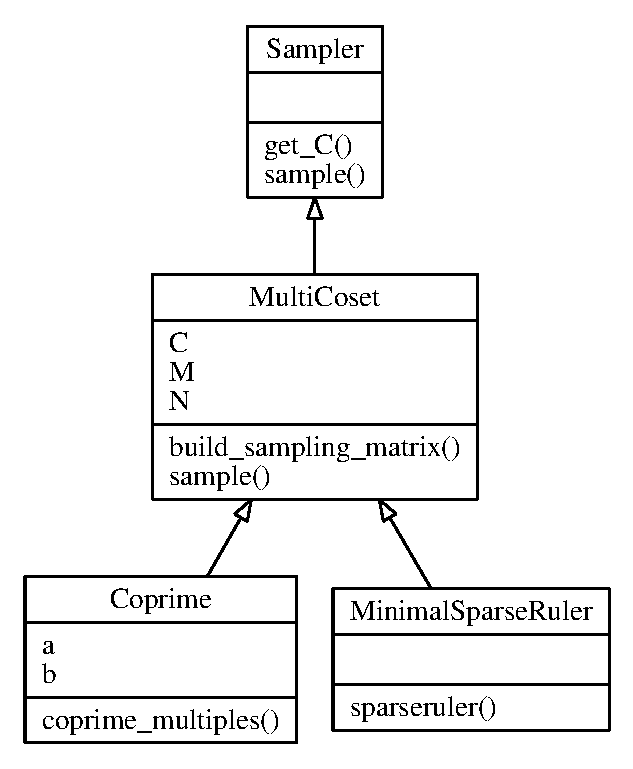
\includegraphics[width=0.5\linewidth]{./figures/classes_sampling.eps}
    \caption{The UML diagram of the samplers}
    \label{fig:umlclasses}
\end{figure}

\subsection{Multi-coset sampler}
\label{sub:multi_coset_sampler}
Multi-coset sampling (as introduced in \cref{cha:sampling}) is based on a multiple device sampler. The crucial component here is the offset of the common sampling period (sometimes referred to as the `ruler' of a multi-coset system in context of the minimal sparse ruler problem). The list of offsets is one of the constructor arguments used to generate the $C$-matrix which has dimensions defined by $M$ and $N$, which are the other arguments of this implementation.

The implementation of the sample method takes a signal, uniformly sampled, as argument and returns a multi-coset sampled signal. Our initial implementation used a loop and a matrix multiplication. To speed up this function the for loop was vectorized by a single matrix multiplication. This is achieved by reshaping the input signal to a matrix with one dimension $N$ and the other determined by the length of the input signal.

\subsection{Minimal sparse ruler sampler}
\label{sec:multi-coset-sampler}
The minimal sparse ruler inherits from the multi-coset sampler. It feeds a solution to the minimal sparse ruler to the multi-coset sampler, which it obtains from a lookup table. It inherits all the other functionality from the multi-coset sampler.

\subsection{Coprime sampler}
\label{sec:coprime-sampler}
The coprime sampler also inherits from the multi-coset sampler. It generates a number of coprime multiples (see \cref{sec:coprime}) as a set of intervals and feeds that into the multi-coset sampler. It inherits all the other functions from the multi-coset sampler.

\subsection{Hardware coprime}
\label{sec:hardware-coprime}
The hardware coprime sampler uses two input sample vectors, with a different number of samples from two samplers with different sample rates. The sampling matrix is constructed as with the normal coprime sampler. The two input vectors are then transformed into one output vector that matches the sampling matrix.

\section{Reconstruction}
\label{sec:reconstruction}
Two different kind of reconstruction methods are implemented. One is similar to the one specified in \cite{ariananda2012compressive} and the other is discussed in \cref{prt:theory} of this thesis. Both reconstructors implement the interface \class{Reconstructor}, which has a contract for a reconstruct-method\footnote{Meaning they should implement such a method.}, which is depicted by the UML-diagram in \cref{fig:umlreconstructor}.

\begin{figure}[h]
    \centering
    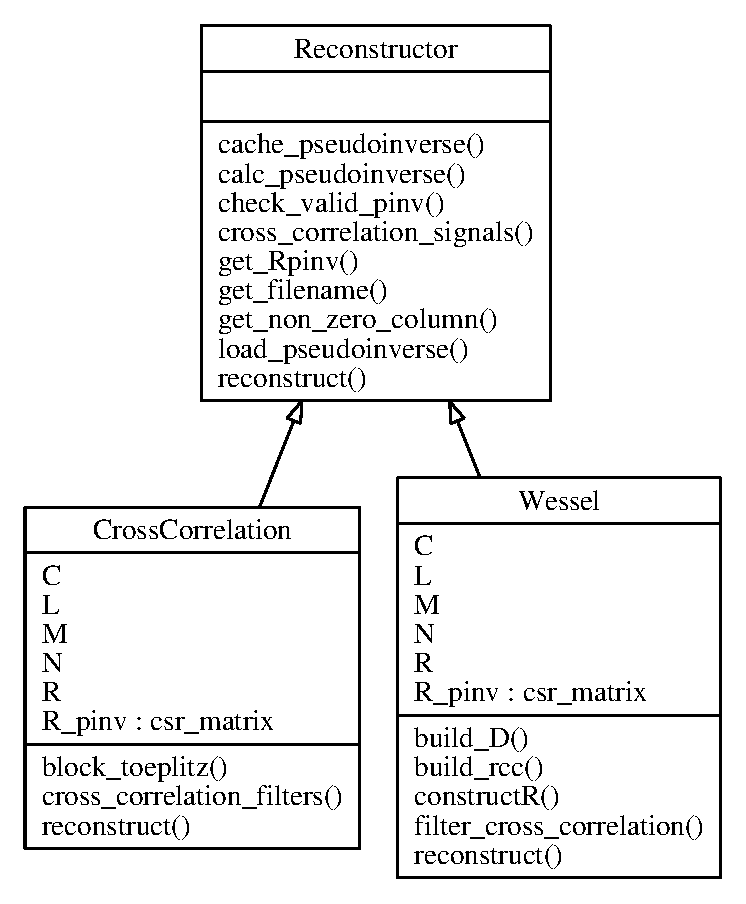
\includegraphics[width=0.5\linewidth]{./figures/classes_reconstruction.eps}
    \caption{The UML diagram of the reconstructors}
    \label{fig:umlreconstructor}
\end{figure}

Both classes make use of shared functionality to calculate a pseudo-inverse. This is a wrapper around \lib{SciPy}'s \func{pinv}. Because this operation is quite time-consuming for larger systems, a caching mechanism was introduced to lower start-up times.

\subsection{CrossCorrelation}
\label{sub:crosscorrelation}
This class implements an algorithm based on the one described in \cite{ariananda2012compressive}. The algorithm has two parameters. The first one determines the maximum lag that will be estimated of cross-correlation of the cosets, often referred to as $L$. The second one is the sampling matrix used by the sampler described in \cref{sec:sampling}. These are also the parameters specified\footnote{\label{fn:reconparam}There are actually four parameters: $L$, $N$, $M$ and $C$. However, $N$ and $M$ can be determined from the shape of $C$.} in the paper.

Optionally a switch can be passed to disable the caching mechanism described in the base class. During the initialisation of the class it builds the $R$-matrix as discussed in \cite{ariananda2012compressive} and computes its pseudo-inverse.

The reconstruct method is implemented by calculating the cross correlations of the non-uniformly sampled input signal. A helper function is defined in the \func{Reconstructor} interface that calculates the cross correlations of the input. To speed up this function the multiple correlations are vectorized into a number of matrix multiplications. The pseudo-inverse is then multiplied by these cross-correlations to reconstruct the signal.

\subsection{Wessel}
\label{sub:wessel}
The Wessel reconstructor is a variation on the reconstruction technique implemented by \class{CrossCorrelation}. The theory is thoroughly described in \cref{prt:theory} of this thesis. The algorithm takes the same parameters\footnoteref{fn:reconparam}, namely the maximum lag estimated of cross-correlation of the cosets and the sampling matrix used by one the non-uniform sampler. This is required for the reconstruction algorithm.

Similar to the other reconstructor implementation, a switch to disable the caching mechanism has been implemented. Like the other reconstructor, this reconstructor generates an $R$-matrix and computes its pseudo-inverse. Details on this algorithm may be found in \cref{cha:reconstruction}.

The reconstruct method is implemented by calculating the cross correlations (again) of the non-uniformly sampled input and multiplying it with the pseudo-inverse.

From an implementation perspective, the structure of the pseudo-inverse of the Wessel algorithm maps better on the data structures of \lib{NumPy}. \lib{NumPy}'s basic array data structures are in row-major order\footnote{This is the standard way of saving an array in C, two notable exceptions that save their arrays in column major order are \matlab{} and Fortran. Column major order is often called Fortran style.}. The final phase of both reconstruction steps is reshaping the cross-correlation matrix to a single column vector and multiplying it with the pseudo-inverse. This operation is more memory efficient in the Wessel reconstructor.

\section{Detection}
\label{sec:detection}
A single kind of detector is implemented. The strategy pattern is still used because of possible future additions. All detectors have to implement the interface \func{Detector}, which has a contract for a detect method.

\subsection{Ariananda}
\label{sub:ariananda}
The Ariananda detector (named after the writer of \cite{ariananda2012compressive}) implements the theory described in \cref{cha:detection}. It takes $L$, $K$, $C$, $\mat{R}^\dagger$, $\mat{R}_c$, window length and $P_{\text{fa}}$ as its parameters. Its current implementation requires the reconstructor to be \func{Wessel}\footnote{It can also be implemented for \func{CrossCorrelation} but requires some adjustments. This has not been implemented.}.

It implements the detect method by calculating a threshold (referred to as $\gamma_k$ in the theory) and comparing that with the PSD of the signal. It makes use of information of the wessel reconstructor and the sampler in question to make a better estimate of a threshold for the signal.


\begin{figure}
    \centering
    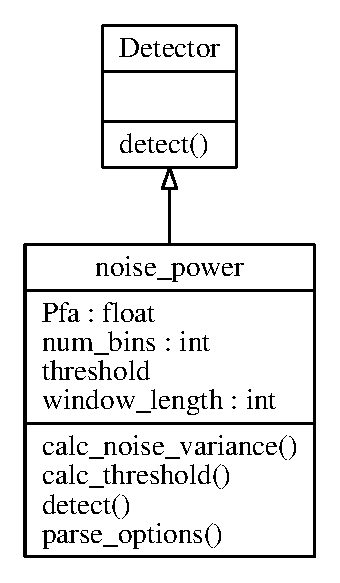
\includegraphics[width=0.5\linewidth]{./figures/classes_detection.eps}
    \caption{The UML diagram of the detectors}
    \label{fig:umldetector}
\end{figure}

\end{document}
